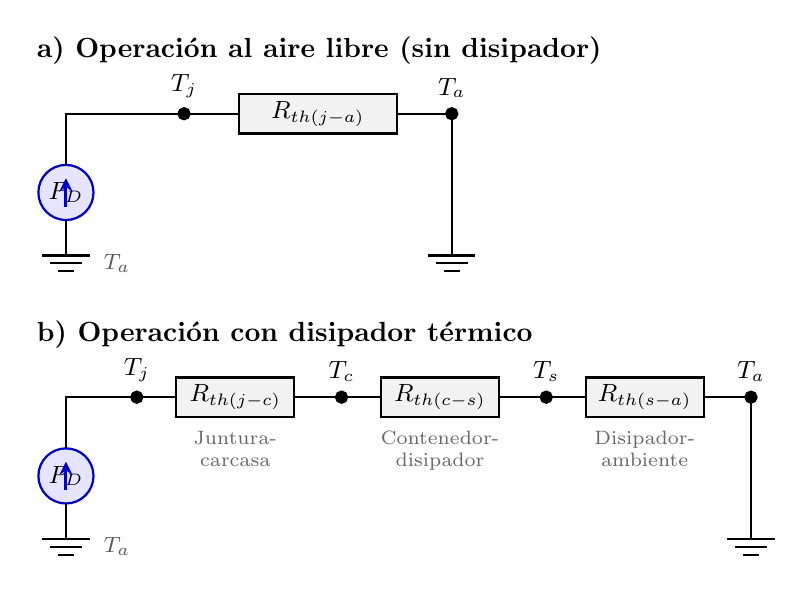
\begin{tikzpicture}[>=stealth, font=\small, thick]
    % --- PARTE A: Sin disipador ---
    \begin{scope}[shift={(0,3.6)}]
        \node[anchor=west, font=\bfseries] at (-0.5, 1.8) {a) Operación al aire libre (sin disipador)};
        
        % Fuente de calor PD
        \filldraw[fill=blue!10, draw=blue!80!black] (0,0) circle (0.35);
        \node at (0,0) {$P_D$};
        \draw[->, line width=1.1pt, color=blue!80!black] (0,-0.18) -- (0,0.18);
        
        % Masa Ta izquierda
        \draw (0,-0.35) -- (0,-0.8);
        \draw (-0.3,-0.8) -- (0.3,-0.8);
        \draw (-0.2,-0.9) -- (0.2,-0.9);
        \draw (-0.1,-1.0) -- (0.1,-1.0);
        \node[anchor=west, font=\footnotesize, text=gray!70!black] at (0.35,-0.9) {$T_a$};
        
        % Conexion a Tj
        \draw (0,0.35) -- (0,1.0) -- (1.5,1.0);
        \filldraw (1.5,1.0) circle (2pt) node[above=2pt] {$T_j$};
        
        % Resistor Rth(j-a)
        \draw (1.5,1.0) -- (2.2,1.0);
        \draw[fill=gray!10] (2.2,0.75) rectangle (4.2,1.25);
        \node at (3.2,1.0) {$R_{th(j-a)}$};
        \draw (4.2,1.0) -- (4.9,1.0);
        \filldraw (4.9,1.0) circle (2pt) node[above=2pt] {$T_a$};
        
        % Masa Ta derecha
        \draw (4.9,1.0) -- (4.9,-0.8);
        \draw (4.6,-0.8) -- (5.2,-0.8);
        \draw (4.7,-0.9) -- (5.1,-0.9);
        \draw (4.8,-1.0) -- (5.0,-1.0);
    \end{scope}

    % --- PARTE B: Con disipador ---
    \begin{scope}[shift={(0,0)}]
        \node[anchor=west, font=\bfseries] at (-0.5, 1.8) {b) Operación con disipador térmico};
        
        % Fuente de calor PD
        \filldraw[fill=blue!10, draw=blue!80!black] (0,0) circle (0.35);
        \node at (0,0) {$P_D$};
        \draw[->, line width=1.1pt, color=blue!80!black] (0,-0.18) -- (0,0.18);
        
        % Masa Ta izquierda
        \draw (0,-0.35) -- (0,-0.8);
        \draw (-0.3,-0.8) -- (0.3,-0.8);
        \draw (-0.2,-0.9) -- (0.2,-0.9);
        \draw (-0.1,-1.0) -- (0.1,-1.0);
        \node[anchor=west, font=\footnotesize, text=gray!70!black] at (0.35,-0.9) {$T_a$};
        
        % Conexion a Tj
        \draw (0,0.35) -- (0,1.0) -- (0.9,1.0);
        \filldraw (0.9,1.0) circle (2pt) node[above=2pt] {$T_j$};
        
        % Resistor Rth(j-c)
        \draw (0.9,1.0) -- (1.4,1.0);
        \draw[fill=gray!10] (1.4,0.75) rectangle (2.9,1.25);
        \node at (2.15,1.0) {$R_{th(j-c)}$};
        \draw (2.9,1.0) -- (3.5,1.0);
        \filldraw (3.5,1.0) circle (2pt) node[above=2pt] {$T_c$};
        
        % Resistor Rth(c-s) (case to sink)
        \draw (3.5,1.0) -- (4.0,1.0);
        \draw[fill=gray!10] (4.0,0.75) rectangle (5.5,1.25);
        \node at (4.75,1.0) {$R_{th(c-s)}$};
        \draw (5.5,1.0) -- (6.1,1.0);
        \filldraw (6.1,1.0) circle (2pt) node[above=2pt] {$T_s$};
        
        % Resistor Rth(s-a) (sink to ambient)
        \draw (6.1,1.0) -- (6.6,1.0);
        \draw[fill=gray!10] (6.6,0.75) rectangle (8.1,1.25);
        \node at (7.35,1.0) {$R_{th(s-a)}$};
        \draw (8.1,1.0) -- (8.7,1.0);
        \filldraw (8.7,1.0) circle (2pt) node[above=2pt] {$T_a$};
        
        % Masa Ta derecha
        \draw (8.7,1.0) -- (8.7,-0.8);
        \draw (8.4,-0.8) -- (9.0,-0.8);
        \draw (8.5,-0.9) -- (8.9,-0.9);
        \draw (8.6,-1.0) -- (8.8,-1.0);
        
        % Anotaciones
        \node[anchor=north, text=gray!80!black, font=\scriptsize, align=center] at (2.15,0.7) {Juntura-\\carcasa};
        \node[anchor=north, text=gray!80!black, font=\scriptsize, align=center] at (4.75,0.7) {Contenedor-\\disipador};
        \node[anchor=north, text=gray!80!black, font=\scriptsize, align=center] at (7.35,0.7) {Disipador-\\ambiente};
    \end{scope}
\end{tikzpicture}
